% DO NOT COMPILE THIS FILE DIRECTLY!
% This is included by the other .tex files.

\begin{frame}[t,plain]
\titlepage
\end{frame}


\begin{frame}
\frametitle{Who are we ?}
    \begin{center}
        
\includegraphics[width=0.3\linewidth]{pictures/circl.png}
    \end{center}
    \begin{itemize}
        \item The Computer Incident Response Center Luxembourg (CIRCL)
        \item CIRCL is the CERT for the private sector, communes and non-governmental entities in Luxembourg
        \item CIRCL leads the development of the open-source MISP threat intelligence platform
        \begin{itemize}
            \item As well as running multiple large MISP communities performain active daily threat-intelligence sharing
        \end{itemize}
    \end{itemize}
\end{frame}

\begin{frame}
\frametitle{MeliCERTes II: a quick recap of the morning session}
    \begin{itemize}
        \item MeliCERTes
        \item Common tooling for CSIRTs
        \item Cerebrate a central component of the new tooling
        \item Takes care of:
        \begin{itemize}
            \item Contact management
            \item orchestration
            \item Sharing group distribution and management
        \end{itemize}
    \end{itemize}
\end{frame}

\begin{frame}
\frametitle{Some stats about one of our MISP instance: MISPPriv (1)}
    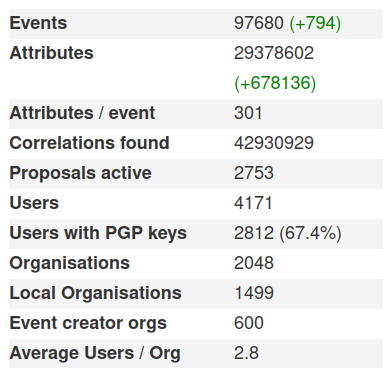
\includegraphics[width=0.45\linewidth]{pictures/misppriv-usage.png}
    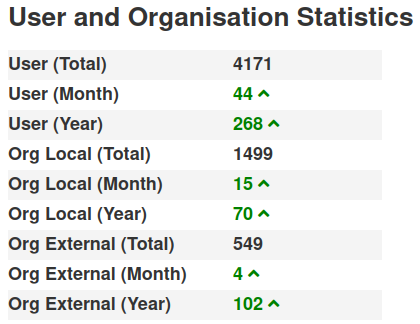
\includegraphics[width=0.45\linewidth]{pictures/misppriv-user-org-stats.png}
\end{frame}

\begin{frame}
    \frametitle{Some stats about one of our MISP instance: MISPPriv (2)}
    \begin{center}
        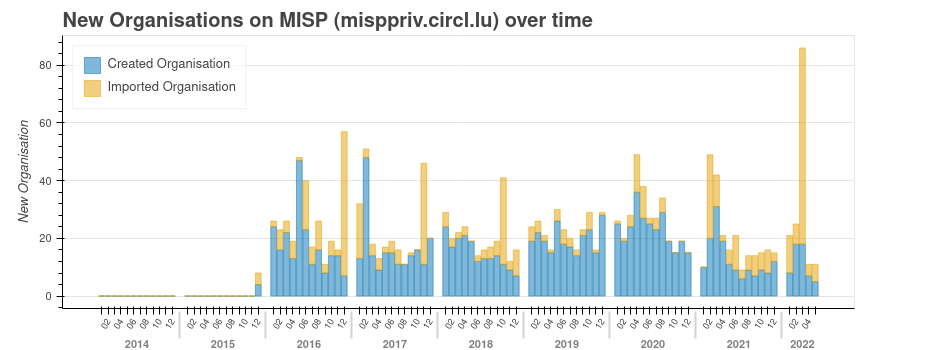
\includegraphics[width=1.1\linewidth]{pictures/bokeh_new_org.png}
    \end{center}
\end{frame}

\begin{frame}
\frametitle{Issues we're trying to solve}
    Rising number of communities is great!
    \begin{itemize}
        \item \textbf{Bridge the gap} between between communities
        \item Sharing with peers that face \textbf{similar threats}
        \item \textbf{Reuse} of TTPs across sectors
        \item \textbf{Hybrid threats} How seemingly unrelated things may be interesting to correlate
        \item \textbf{Spread the love}, as our field is ahead of several other sectors when it comes to information sharing
    \end{itemize}
\end{frame}

\begin{frame}
\frametitle{Issues we're trying to solve}
    However, broader and more diverse communities lead to more issues
    \begin{itemize}
        \item {Non-technical issues}
        \begin{itemize}
            \item Sharing difficulties in terms of social interactions (e.g trust)
            \begin{itemize}
                \item 
\includegraphics[width=80px]{pictures/firstcon-22.png} greatly helps in that aspect!
            \end{itemize}
            \item Lots of points of contacts
        \end{itemize}
    \end{itemize}

    \begin{itemize}
        \item {Technical issues}
        \begin{itemize}
            \item Centralised identity management 
            \item Data might change or evolve over time
            \item Loads of UUIDs to manually process
            \item Distribution list management is difficult across communities
        \end{itemize}
    \end{itemize}
    \begin{center}
        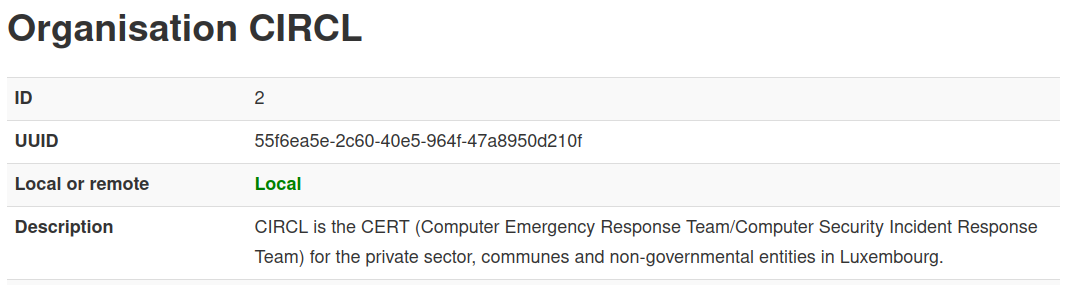
\includegraphics[width=0.8\linewidth]{pictures/org-circl.png}
    \end{center}
\end{frame}

\begin{frame}
\frametitle{Issues we're trying to solve with Cerebrate}
    \begin{minipage}{0.8\textwidth}
        \begin{itemize}
            \item Constituencies of organisations
            \begin{itemize}
                \item Geographic \& sectorial
                \item But also technical: CIDR blocks \& AS Numbers
            \end{itemize}
            \item Cryptographic key lookup for information signing
            \begin{itemize}
                \item MISP's protected event feature (New since MISP v2.4.156)
            \end{itemize}
        \end{itemize}
    \end{minipage}
    \begin{minipage}{0.19\textwidth}
        % 
\includegraphics[width=0.8\linewidth]{pictures/clippy-hint.png}
    \end{minipage}
\end{frame}

\begin{frame}
\frametitle{Issues we're trying to solve with Cerebrate}
    \begin{minipage}{0.8\textwidth}
        \begin{itemize}
            \item Constituencies of organisations
            \begin{itemize}
                \item Geographic \& sectorial
                \item But also technical: CIDR blocks \& AS Numbers
            \end{itemize}
            \item Cryptographic key lookup for information signing
            \begin{itemize}
                \item MISP's protected event feature (New since MISP v2.4.156)
            \end{itemize}
        \end{itemize}
    \end{minipage}
    \begin{minipage}{0.19\textwidth}
        
\includegraphics[width=0.8\linewidth]{pictures/clippy-hint.png}
    \end{minipage}
\end{frame}

\begin{frame}
\frametitle{Issues we're trying to solve with Cerebrate}
    \begin{itemize}
        \item Customisable data model adaptable to each community
        \begin{itemize}
            \item Based on the sheer amount of different types of communities, \textbf{it's a must}
        \end{itemize}
        \item Sharing group management
        \item Synchronisation and lookup system
    \end{itemize}
\end{frame}

\begin{frame}
\frametitle{Our attempt at solving them: Cerebrate}
    \begin{itemize}
        \item Open source community management and orchestration tool
    \end{itemize}
    \begin{center}
        
\includegraphics[width=0.15\linewidth]{pictures/logo.png}
        \linebreak
        
\includegraphics[width=0.99\linewidth]{pictures/cerebrate-github.png}
    \end{center}
    \begin{itemize}
        \item Central tool for the \textbf{Melicertes 2 project} (Co-funded by the EU as a CEF project - SMART 2018/1024)
        \item Rich \textbf{Contact Database}
        \item Tightly coupled management system and companion for MISP (and other tools)
        \begin{itemize}
            \item Get in touch with us if you need help building integrations!
        \end{itemize}
        \item Planned as the primary MISP \textbf{fleet management} tool
    \end{itemize}
\end{frame}

\begin{frame}
\frametitle{Goals and design}
    \begin{itemize}
        \item Goals: Simplicity, lightweight and open-source
        \item Technologies used: PHP, cakephp4, BS5, ...
            \begin{itemize}
                \item (almost) the same as in MISP for easier \textbf{maintainability} and \textbf{code re-use}
            \end{itemize}
        \item IAM centric design
            \begin{itemize}
                \item Tightly integrated with Keycloak
            \end{itemize}
        \item Core functionalities: Auditing, API
            \begin{itemize}
                \item Any changes should be easily accessible to counter errors or foul plays
                \item From our perspective, automation and integration is essential and should be as easy as possible
            \end{itemize}
    \end{itemize}
\end{frame}

\begin{frame}
\frametitle{Goals and design}
    \begin{itemize}
        \item Built with tool integration in mind, acting as a contact database
    \end{itemize}
    \begin{center}
        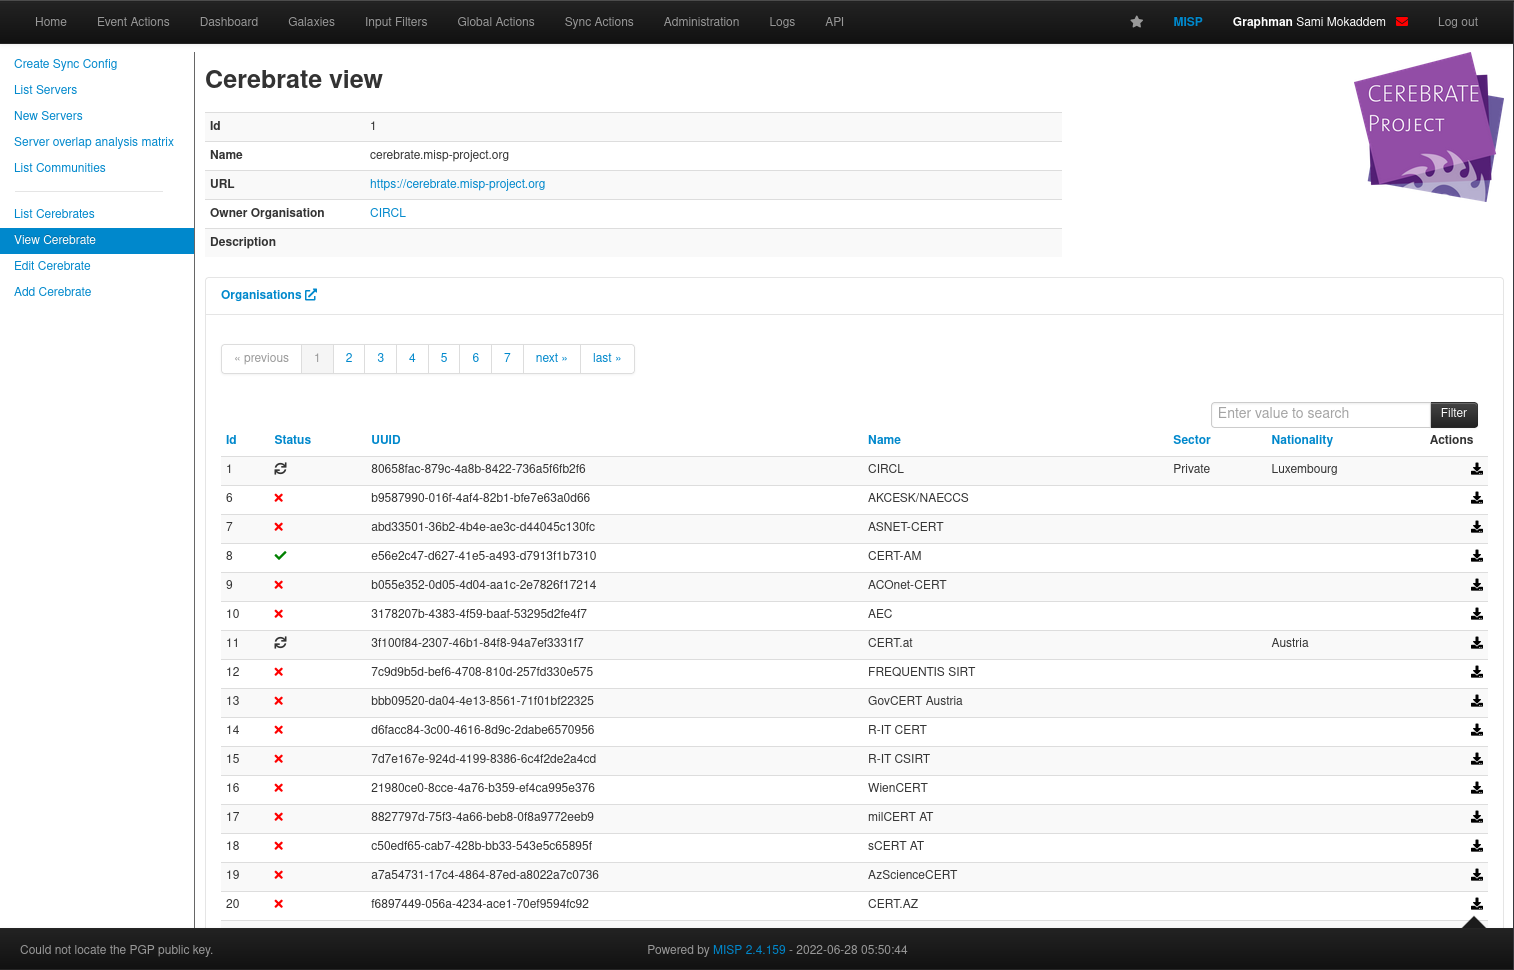
\includegraphics[width=0.85\linewidth]{pictures/misp-cerebrate.png}\\

        MISP is able to look up Organisations \& Sharing Group in Cerebrate
    \end{center}
\end{frame}

\begin{frame}
\frametitle{Cerebrate's place in a typical CSIRT software stack}
    \begin{center}
        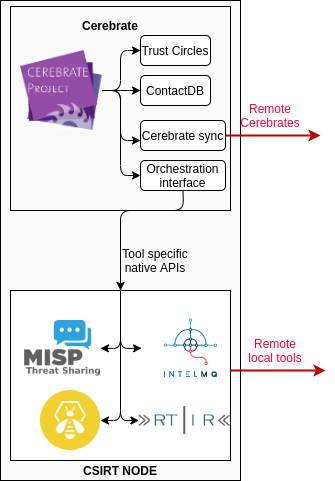
\includegraphics[width=0.42\linewidth]{pictures/software-stack.png}
    \end{center}
\end{frame}

\begin{frame}
\frametitle{Cerebrate's contact database}
    \begin{itemize}
        \item Contact database for the CSIRT network
        \begin{itemize}
            \item Common contact fields such as \texttt{UUID}, \texttt{name}, \texttt{contact email address}, \texttt{nationality}, \texttt{URL}, ...
        \end{itemize}
    \end{itemize}
    \begin{center}
        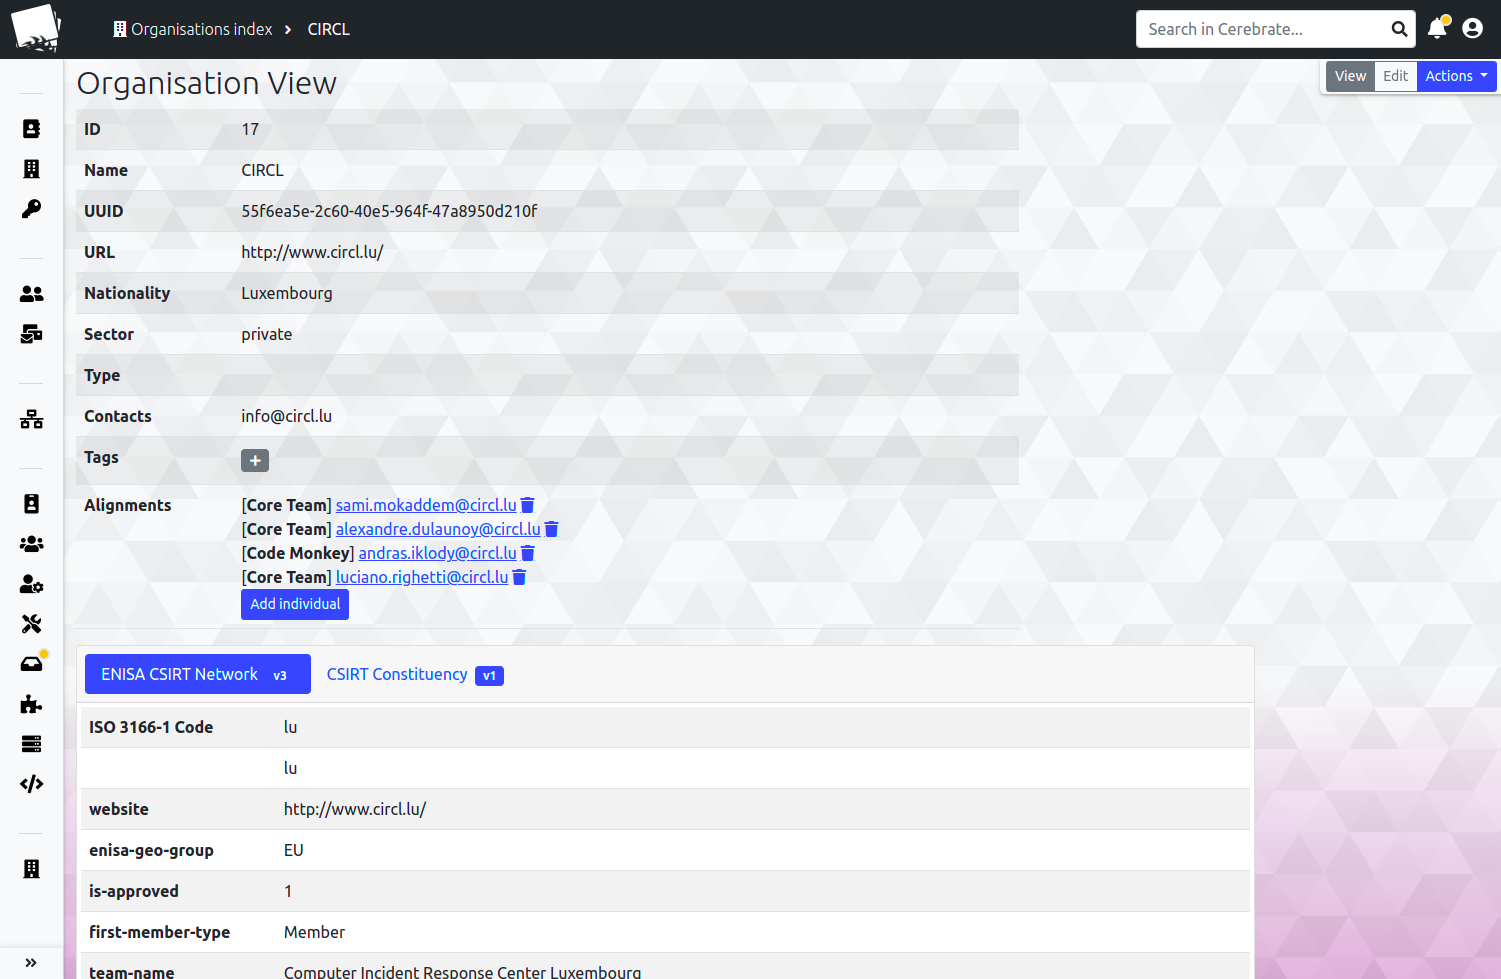
\includegraphics[width=0.8\linewidth]{pictures/contact-database-1.png}
    \end{center}
\end{frame}

\begin{frame}
\frametitle{Cerebrate's contact database}
    \begin{center}
        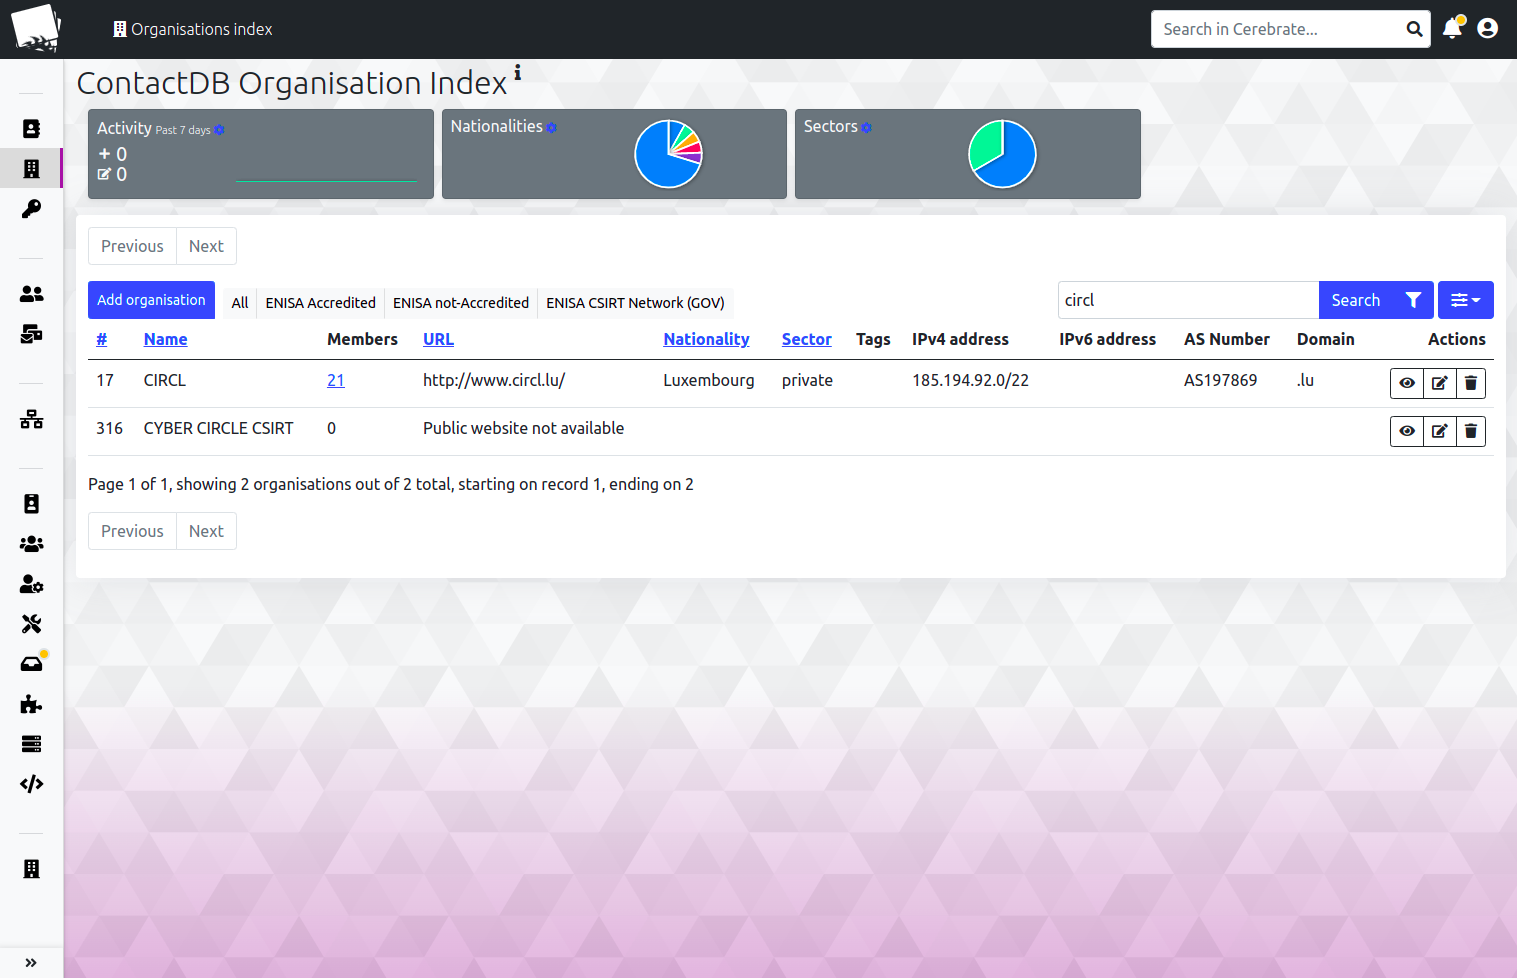
\includegraphics[width=0.99\linewidth]{pictures/contact-database-2.png}
    \end{center}
\end{frame}

\begin{frame}
\frametitle{Cerebrate's contact database: Meta-fields}
    \begin{itemize}
        \item Flexible system to store additional information: \texttt{meta-fields} (KV-store)
        \item These \texttt{meta-fields} are part of a larger structure called \texttt{meta-templates}
        \item Support of multiple templates used by various entities out there
        \begin{itemize}
            \item {\bf FIRST Directory}
            \item ENISA CSIRT inventory
            \item CSIRT Constituency (CIDR blocks, AS Numbers, ...)
        \end{itemize}
    \end{itemize}
\end{frame}

\begin{frame}
\frametitle{Cerebrate's contact database: Meta-fields}
\begin{center}
    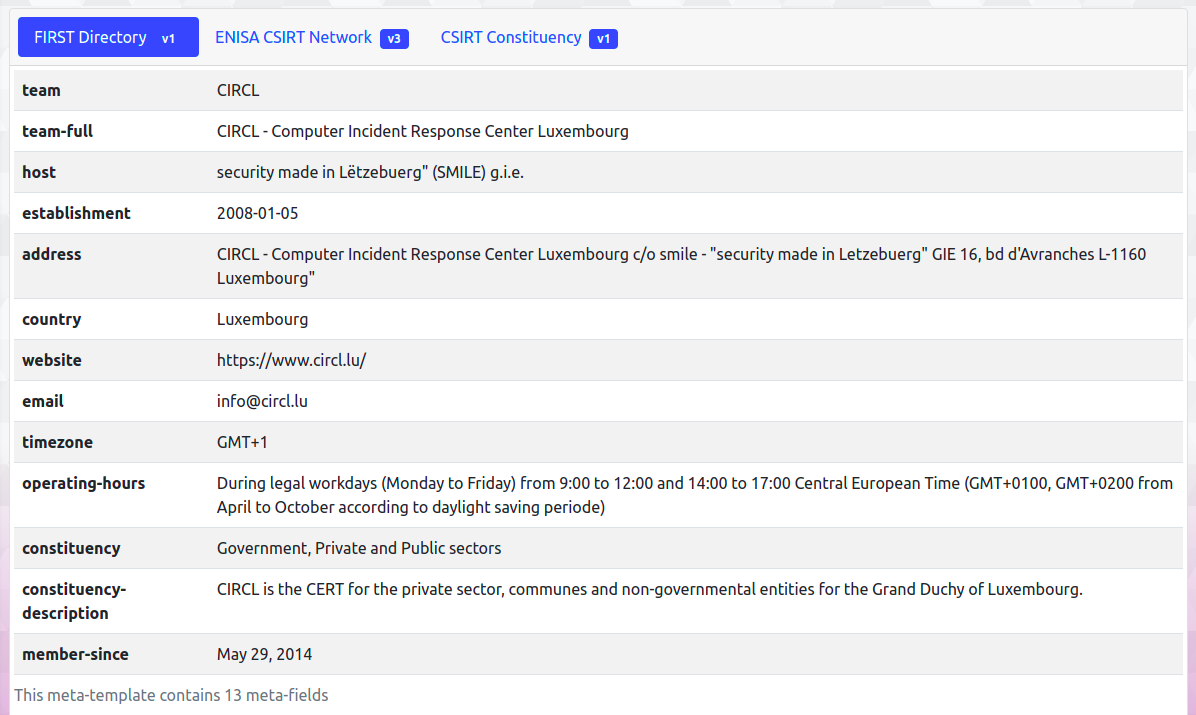
\includegraphics[width=0.99\linewidth]{pictures/meta-fields-first.png}
\end{center}
\end{frame}

\begin{frame}
\frametitle{Cerebrate's contact database: Meta-fields}
\begin{center}
    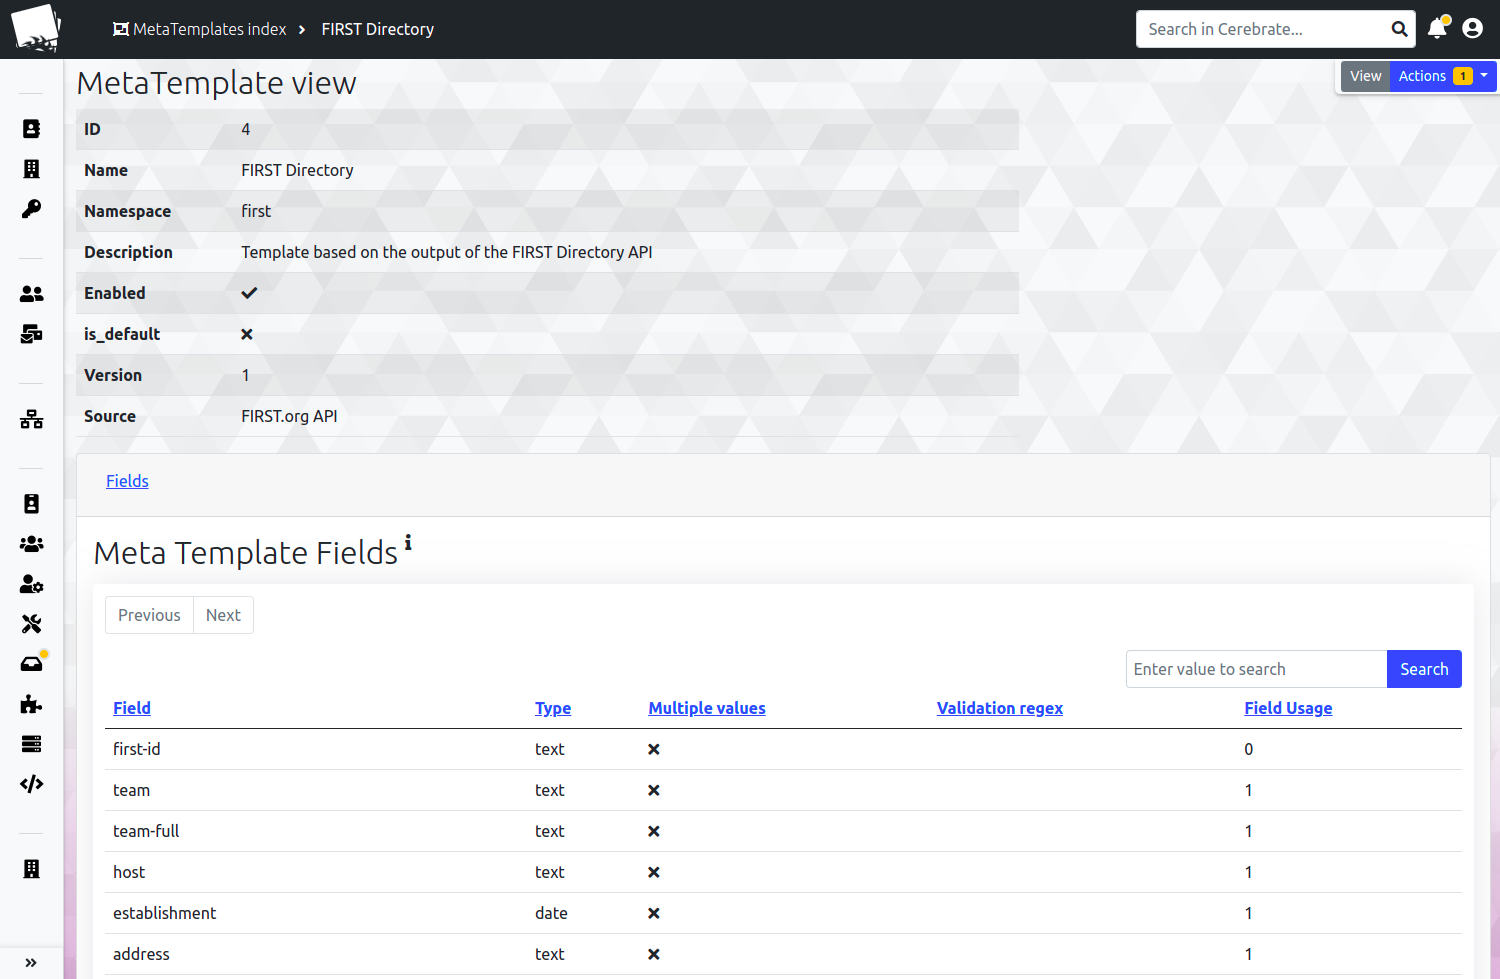
\includegraphics[width=0.99\linewidth]{pictures/meta-templates-first.png}
\end{center}
\end{frame}

\begin{frame}
\frametitle{Cerebrate's contact database: Meta-fields}
\begin{center}
    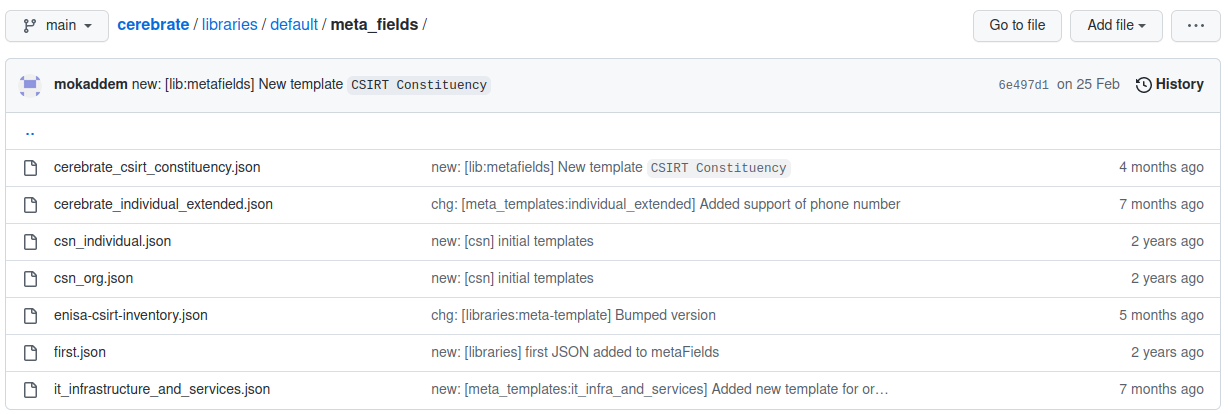
\includegraphics[width=0.99\linewidth]{pictures/meta-template-repo.png}
\end{center}
\end{frame}

\begin{frame}
\frametitle{Cerebrate's contact database: Sharing group management}
    \begin{itemize}
        \item Easy way to \textbf{create} and \textbf{share} distribution lists
        \item Allow sharing groups to be \textbf{reusable}
        \item Circumvent limitations of traditional Threat Intelligence Sharing Platform
        \begin{itemize}
            \item The exchange of sharing groups on creation / modification rather than on data exchange
            \item Avoids the duplication of similar sharing groups
        \end{itemize}
    \end{itemize}
\end{frame}

\begin{frame}
\frametitle{Cerebrate's contact database: Sharing group management}
    \begin{center}
        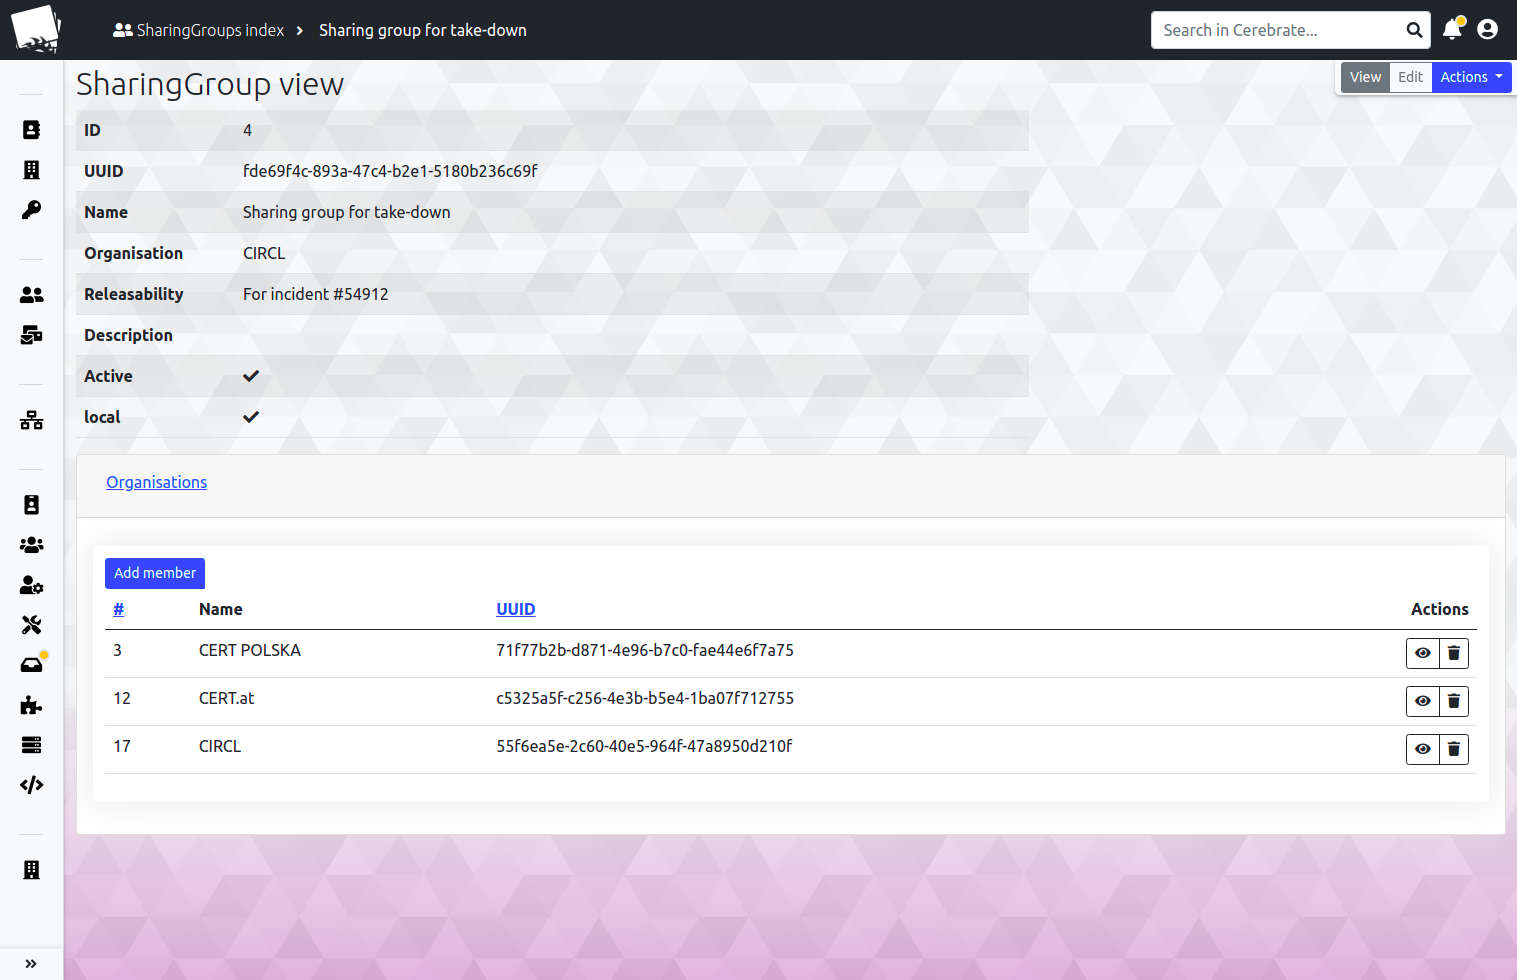
\includegraphics[width=0.9\linewidth]{pictures/sharinggroup.png}
    \end{center}
\end{frame}

\begin{frame}
\frametitle{Cerebrate's contact database: Identity and Signing}
    \begin{itemize}
        \item Cerebrate can act as a trusted contact database containing cryptographic keys (PGP, S/MIME)
        \item Which can be used by other application to sign and validate information
        \begin{itemize}
            \item See MISP's protected Event feature 
\includegraphics[width=0.09\linewidth]{pictures/clippy-solo.png}
        \end{itemize}
    \end{itemize}
\end{frame}

\begin{frame}
\frametitle{Cerebrate's contact database: Identity and Signing}
    \begin{center}
        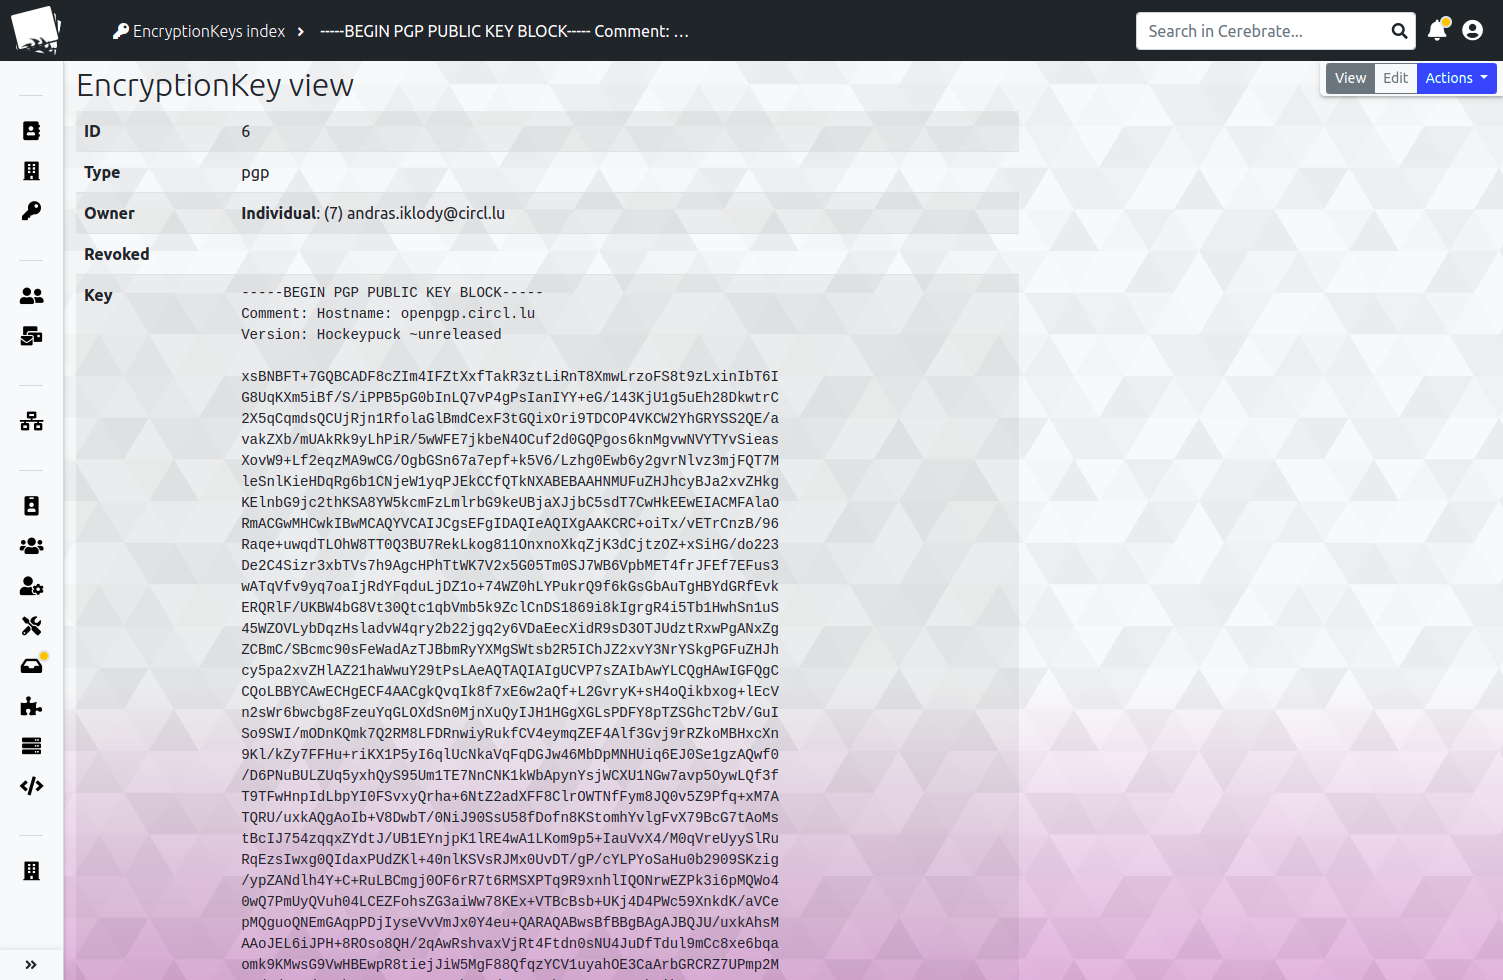
\includegraphics[width=0.95\linewidth]{pictures/pgp.png}
    \end{center}
\end{frame}

\begin{frame}
\frametitle{Cerebrate's contact database: Open Directory}
    \begin{itemize}
        \item Cerebrate can be configured to act as an \textbf{open} directory of contact information
        \item Other tools (including other Cerebrate nodes) can use this directory
        \item Allows for information and information source validation
    \end{itemize}
    \begin{center}
        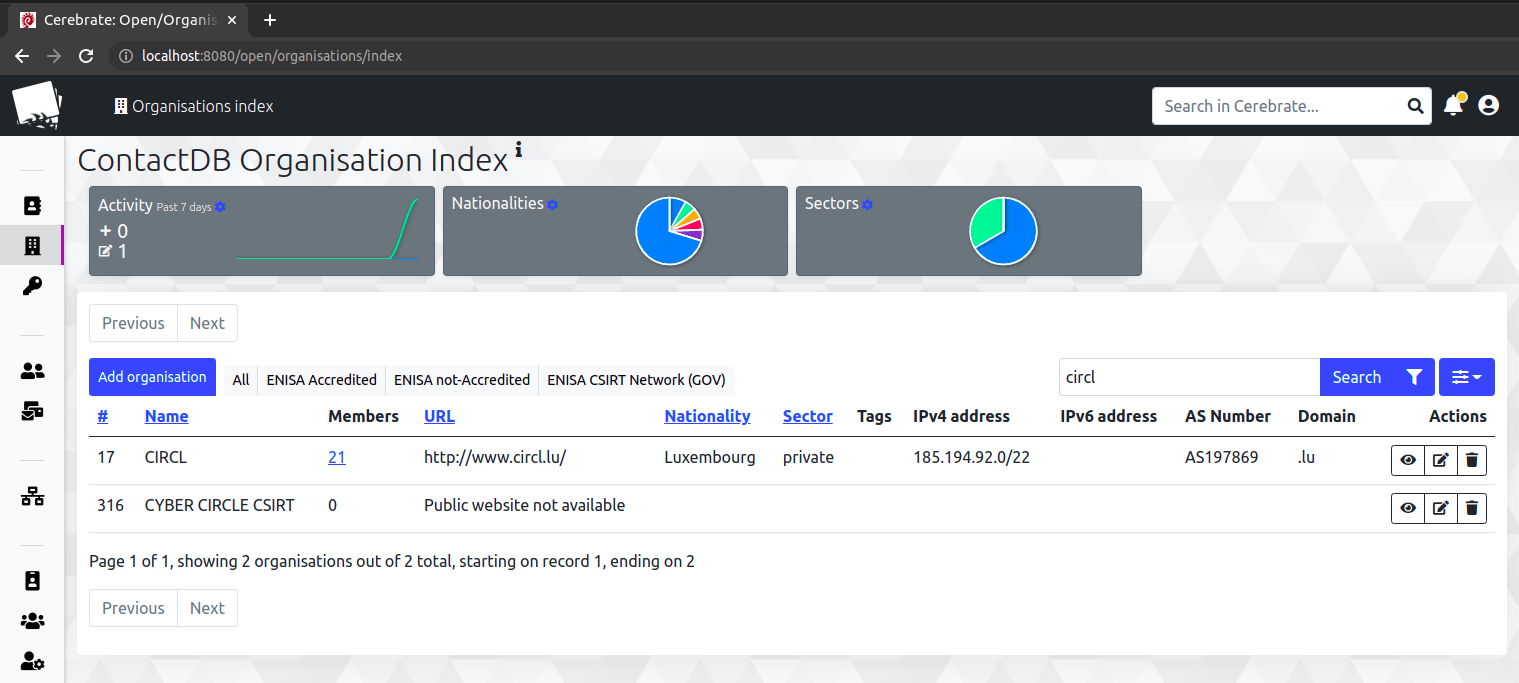
\includegraphics[width=0.8\linewidth]{pictures/open-directory.png}
    \end{center}
\end{frame}

\begin{frame}
\frametitle{Data sharing}
Basically the same strategy as the one used in MISP:
    \begin{itemize}
        \item \textbf{Connect} with other Cerebrate nodes
        \item \textbf{Diagnose} connectivity issues
        \item Remotely \textbf{browse} data of the other node
        \item \textbf{Fetch and save} organisation, individual, sharing-group data
    \end{itemize}
\end{frame}

\begin{frame}
\frametitle{Data sharing}
    \begin{center}
        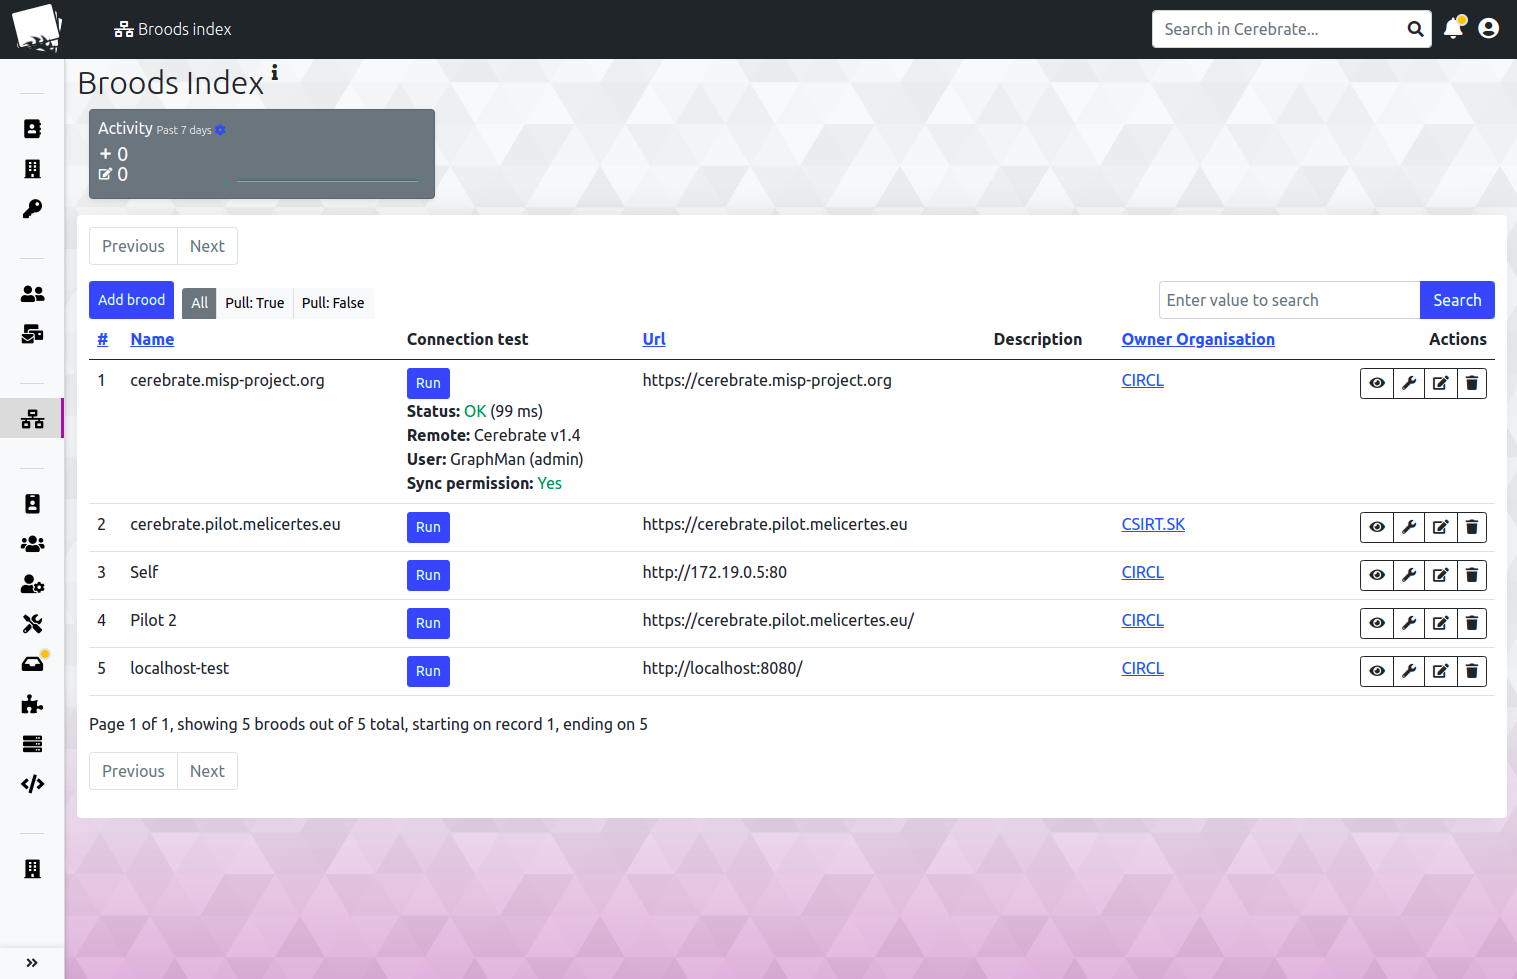
\includegraphics[width=0.95\linewidth]{pictures/brood-index.png}
    \end{center}
\end{frame}

\begin{frame}
\frametitle{Data sharing}
    \begin{center}
        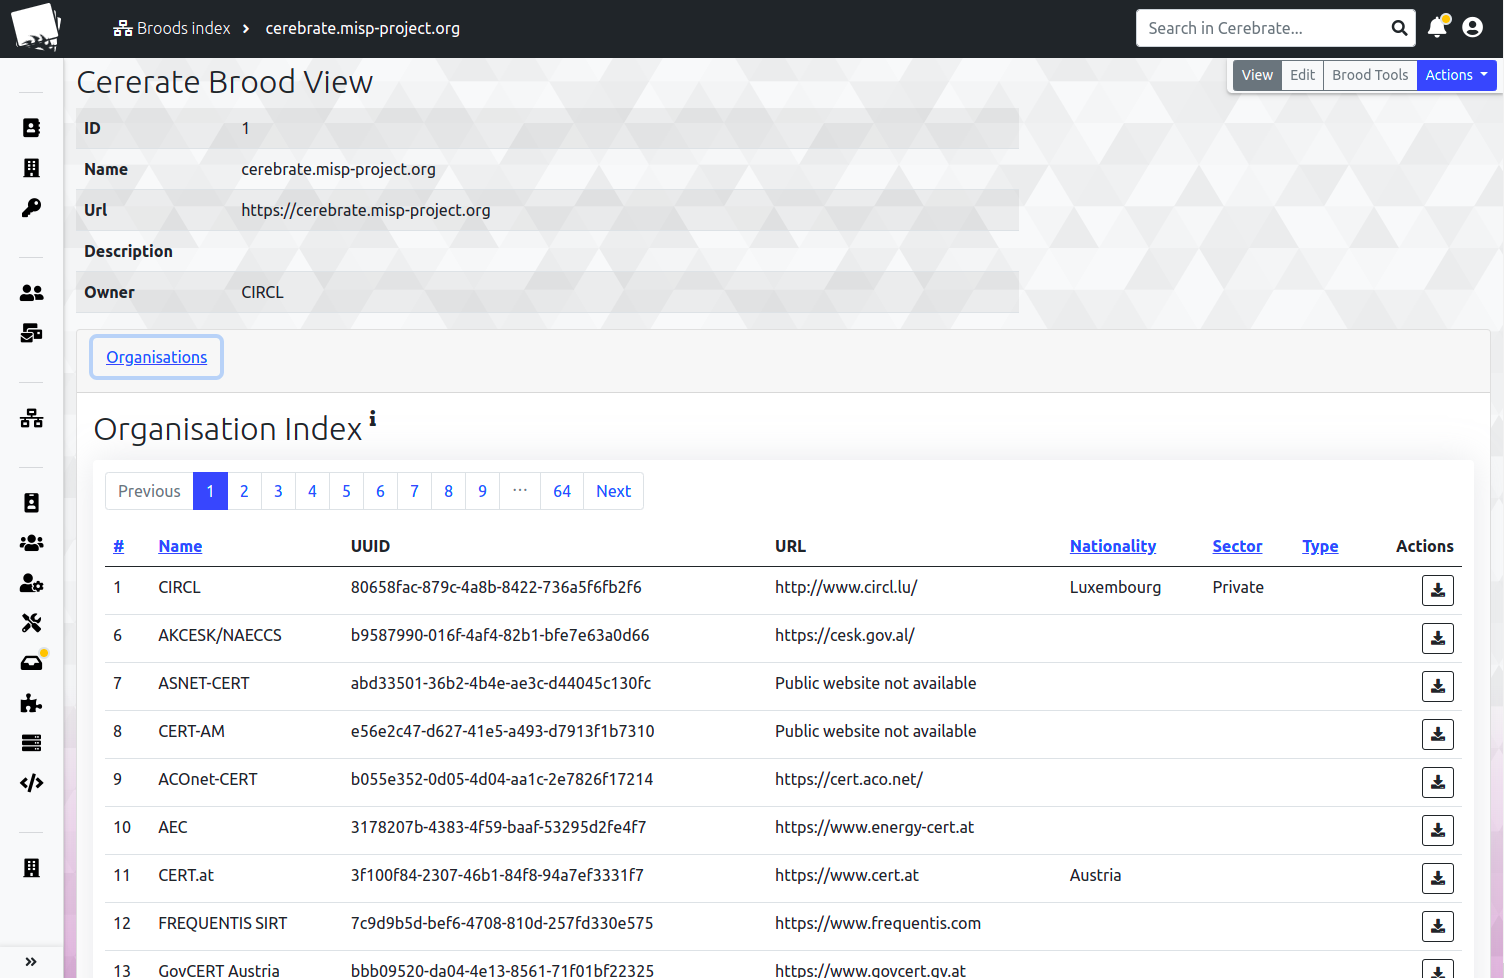
\includegraphics[width=0.95\linewidth]{pictures/brood-view.png}
    \end{center}
\end{frame}

\begin{frame}
\frametitle{Data sharing: Synchronisation strategies}
Two synchronisation strategies:
    \begin{enumerate}
        \item \textbf{Standard}: Only fetch and save new records
        \item \textbf{Trusted upstream source}: Remote Cerebrate acts as an authoritative instance
    \end{enumerate}
    \begin{center}
        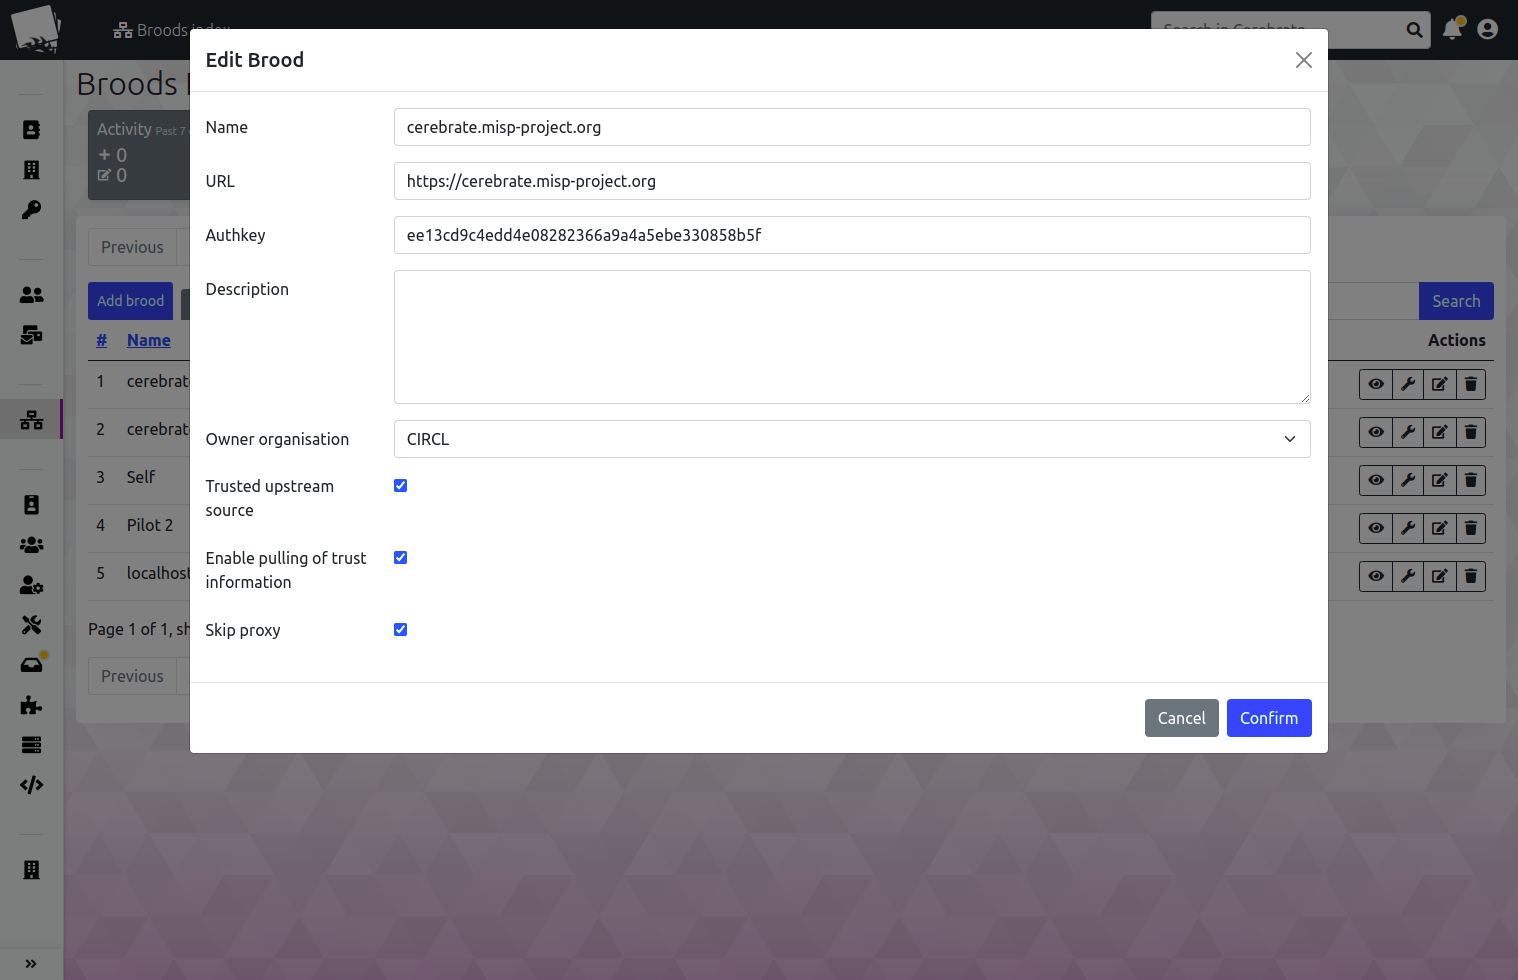
\includegraphics[width=0.7\linewidth]{pictures/brood-edit.png}
    \end{center}
\end{frame}

\begin{frame}
\frametitle{Managing local tools}
Why would Cerebrate have integration with other tools?
    \begin{itemize}
        \item To support information sharing, being able to validate information sources is crucial
        \item Traditional information sharing software stacks have to have their own organisation database
        \item Why re-invent the wheel everytime?
    \end{itemize}
    \begin{center}
        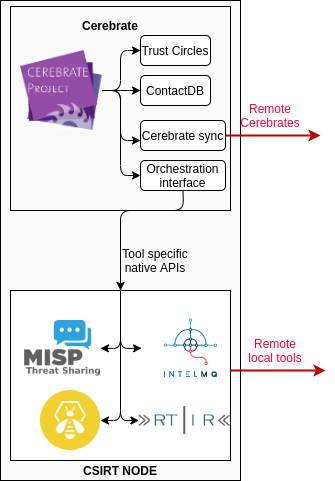
\includegraphics[width=0.2\linewidth]{pictures/software-stack.png}
    \end{center}
\end{frame}

\begin{frame}
\frametitle{Managing local tools}
There will inevitably be integration between local tools and Cerebrate. Why not go a step further?
    \begin{itemize}
        \item Cerebrate exposes a modular system to manage these local tools
        \item Based on a configuration file, user interfaces can be created to visualise data and instruct local tools to perform operations
    \end{itemize}
    \begin{center}
        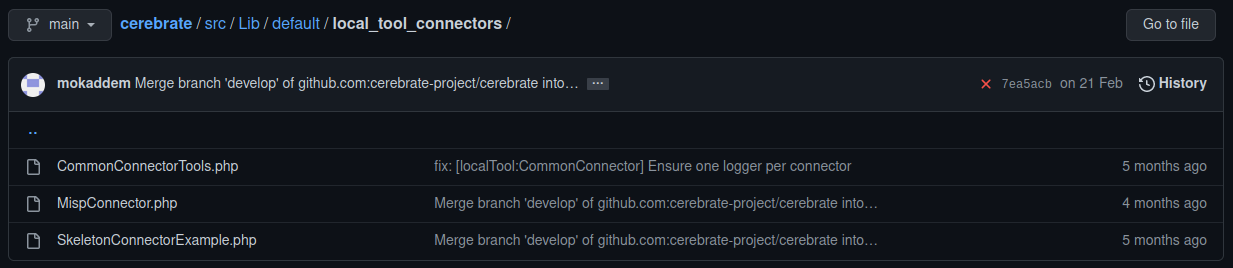
\includegraphics[width=0.7\linewidth]{pictures/github-local-tool.png}
    \end{center}
\end{frame}

\begin{frame}
\frametitle{Local tool: MISP Connector capabilities}
    \begin{itemize}
        \item \textbf{Configure} a MISP instances via server settings
        \item \textbf{Fetch} Organisations \& Sharing Groups
        \item \textbf{Diagnose} other connected MISP servers
        \item \textbf{Manage} users, ...
    \end{itemize}
\end{frame}

\begin{frame}
\frametitle{Local tool: MISP Connector capabilities}
    \begin{center}
        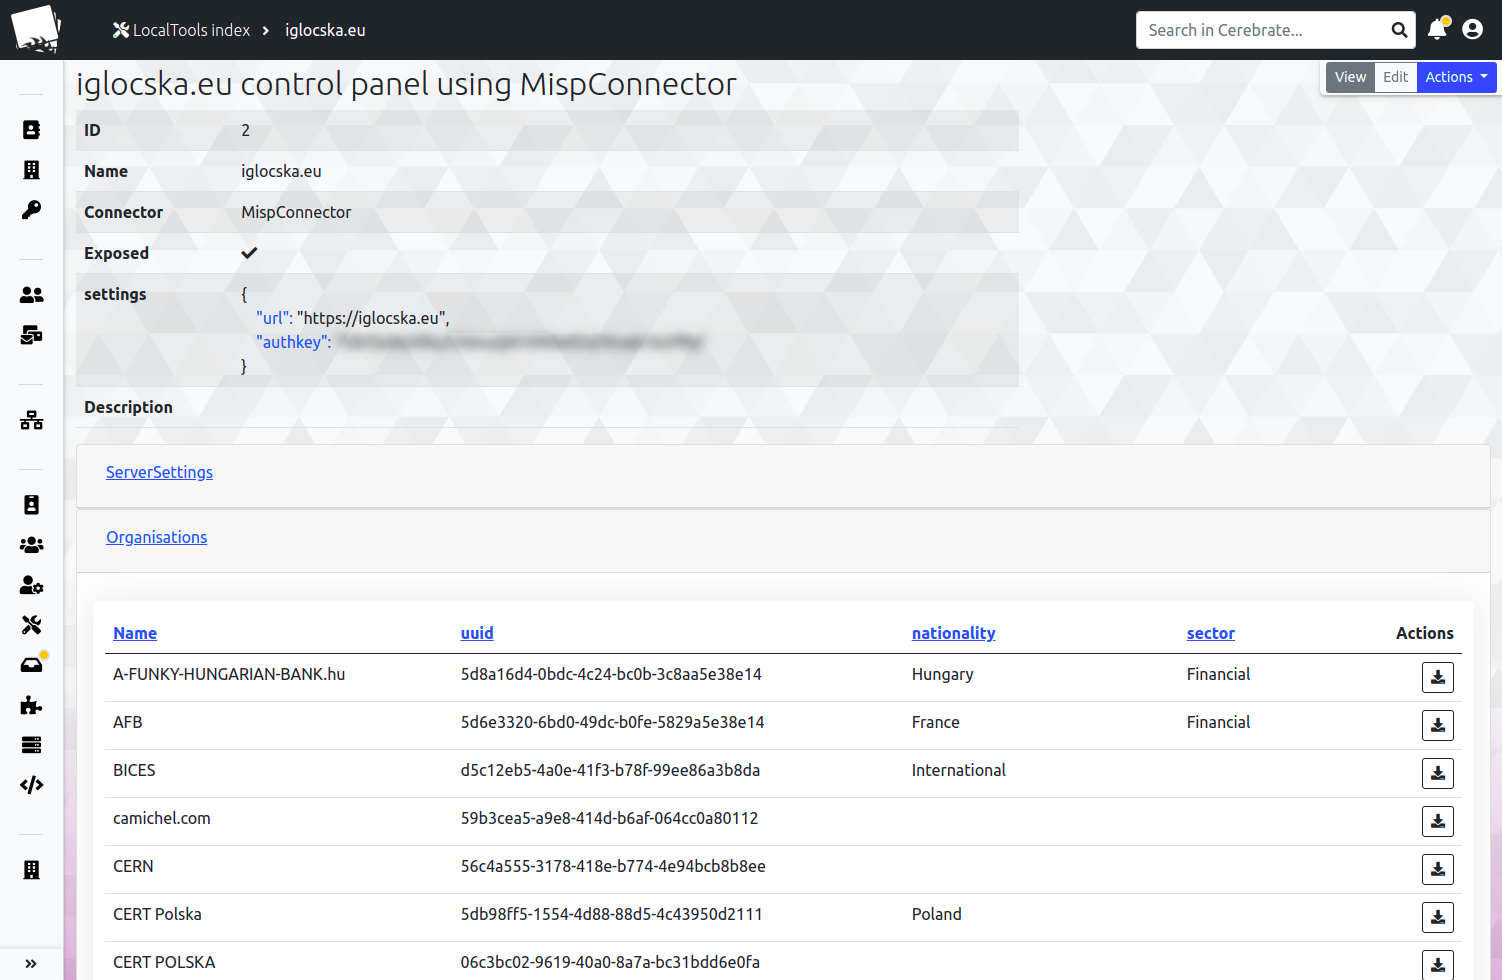
\includegraphics[width=0.97\linewidth]{pictures/localtool-view.png}
    \end{center}
\end{frame}

\begin{frame}
\frametitle{Local tool: MISP Connector capabilities}
    Why do one when we can do many?
    \begin{itemize}
        \item Cerebrate can connect to multiple tools via its associated connector
        \item Allowing local tool fleet management
        \begin{itemize}
            \item MISP fleet management!
        \end{itemize}
    \end{itemize}
\end{frame}

\begin{frame}
    \frametitle{Local tool: MISP Fleet management}
    \begin{center}
        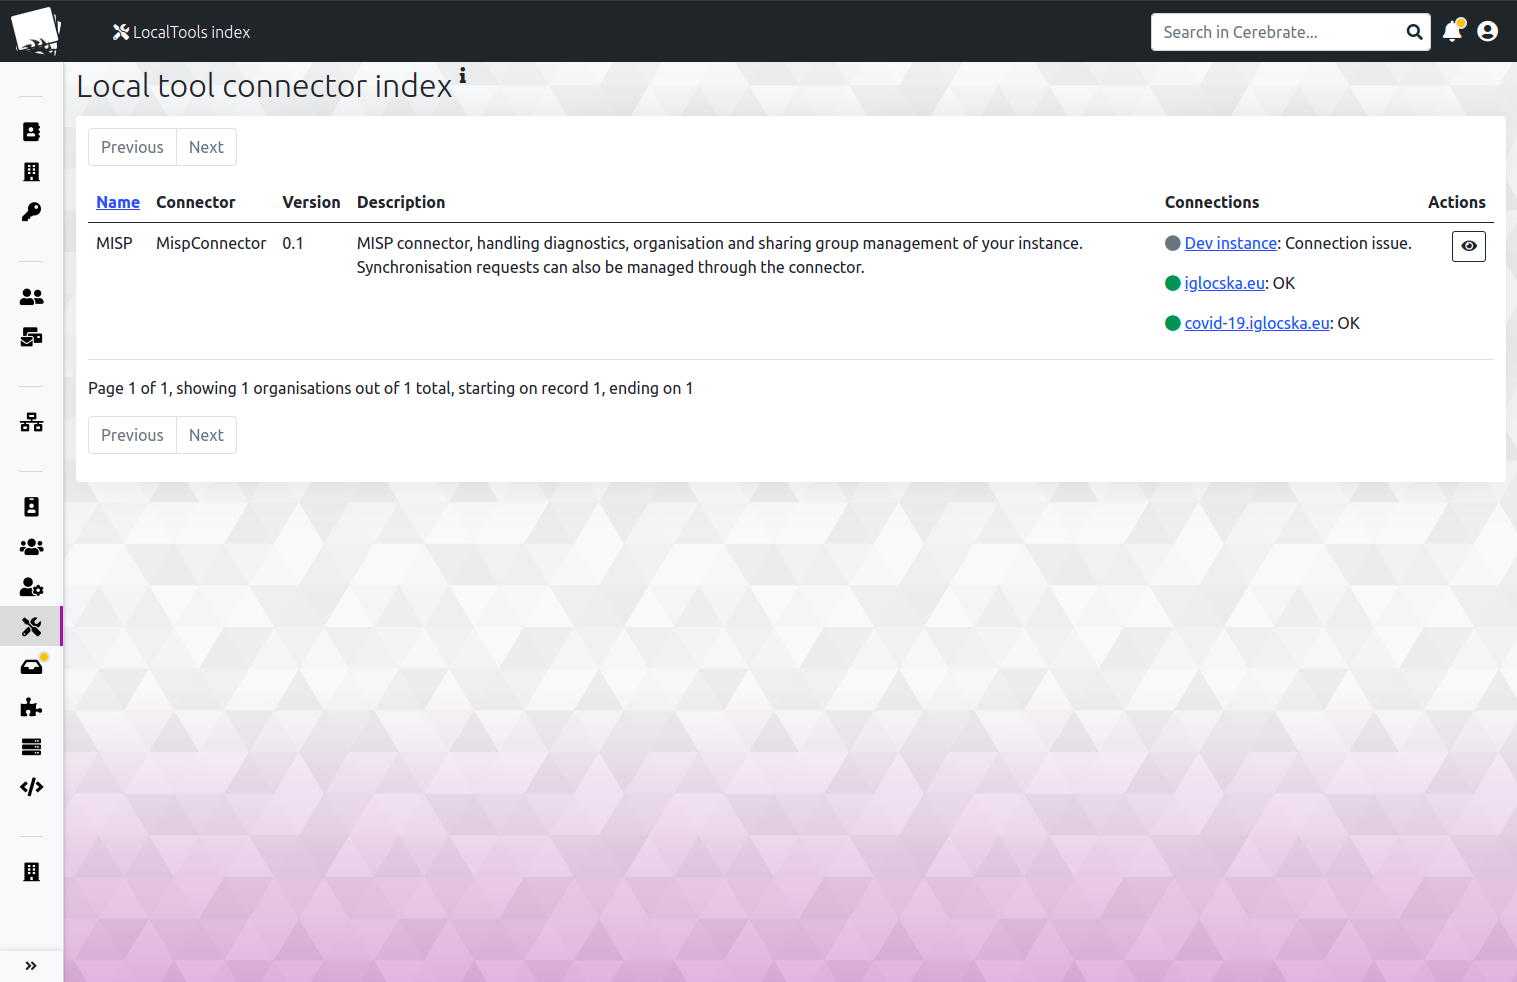
\includegraphics[width=0.97\linewidth]{pictures/localtools-index.png}
    \end{center}
\end{frame}

\begin{frame}
\frametitle{Local tool interconnection via Cerebrate}
    \begin{itemize}
        \item Cerebrate's main goal is to \textbf{ease community management}
        \item Select which local tools are meant to be exposed to the community for requests
        \item Open dialogues to community members to request tool-to-tool interconnections
    \end{itemize}
\end{frame}

\begin{frame}
\frametitle{Local tool interconnection via Cerebrate}
    Cerebrate can leverage its access to local tool to reach out to tools from other Cerebrate nodes
    \begin{center}
        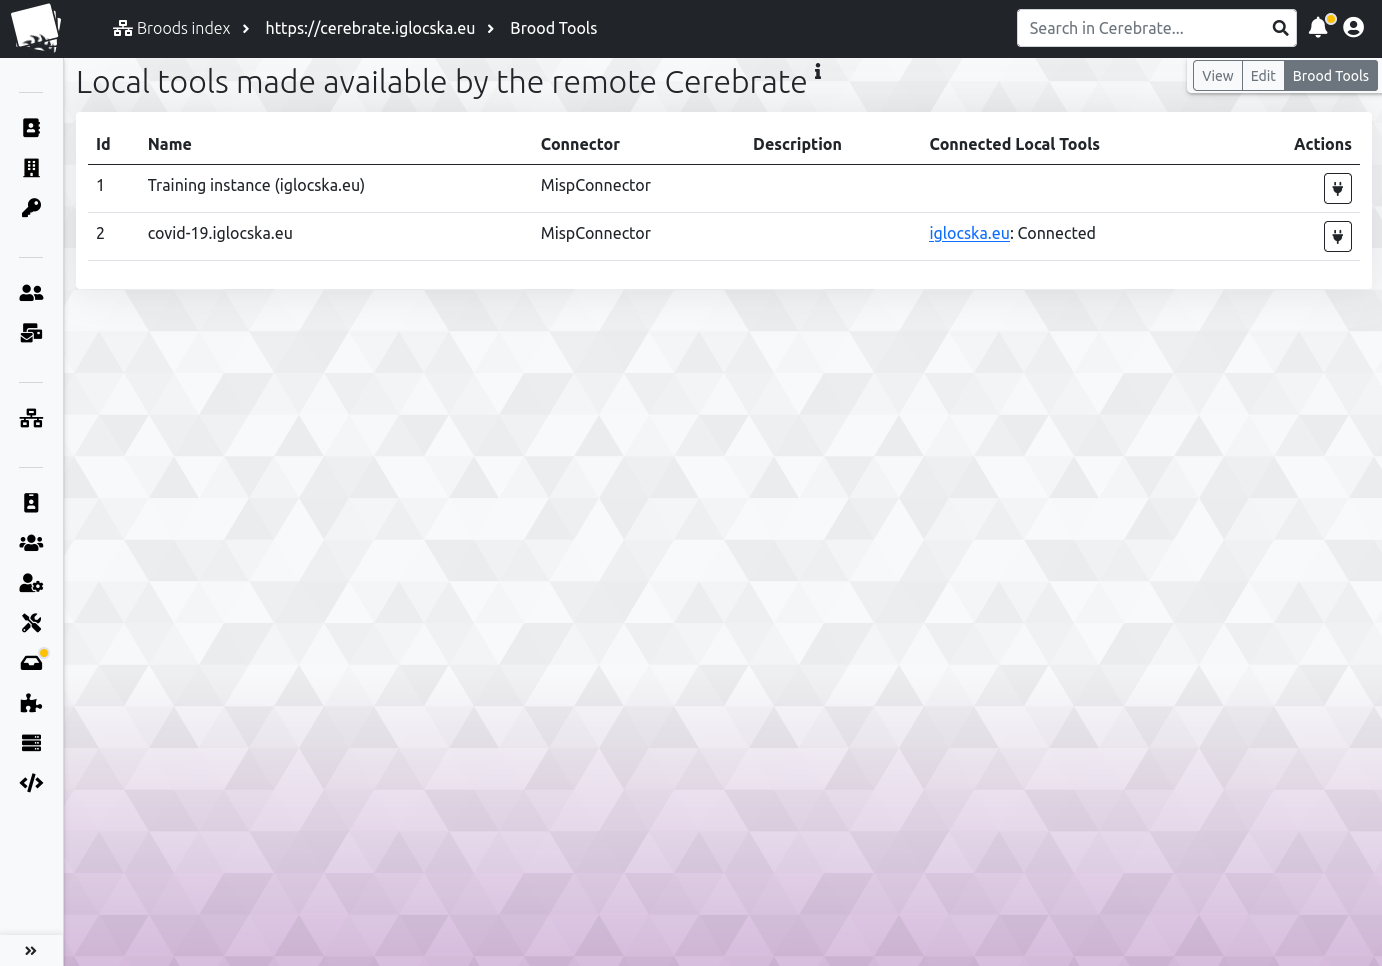
\includegraphics[width=0.85\linewidth]{pictures/tools-made-available.png}
    \end{center}
\end{frame}

\begin{frame}
\frametitle{Local tool interconnection via Cerebrate}
    \begin{itemize}
        \item Local tools can be \textbf{exposed} to other Cerebrate nodes
        \item \textbf{Inter-connection requests} can be issued from one node to another
        \item Following a 3-way handshake protocol, inter-connections can be:
        \begin{itemize}
            \item Issued
            \item Accepted
            \item Finalised
        \end{itemize}
    \end{itemize}
\end{frame}

\begin{frame}
\frametitle{Local tool interconnection via Cerebrate}
    \begin{center}
        
\includegraphics[width=0.40\linewidth]{pictures/guys-chatting.png}
    \end{center}
\end{frame}

\begin{frame}
\frametitle{MISP interconnection via Cerebrate}
    \begin{center}
        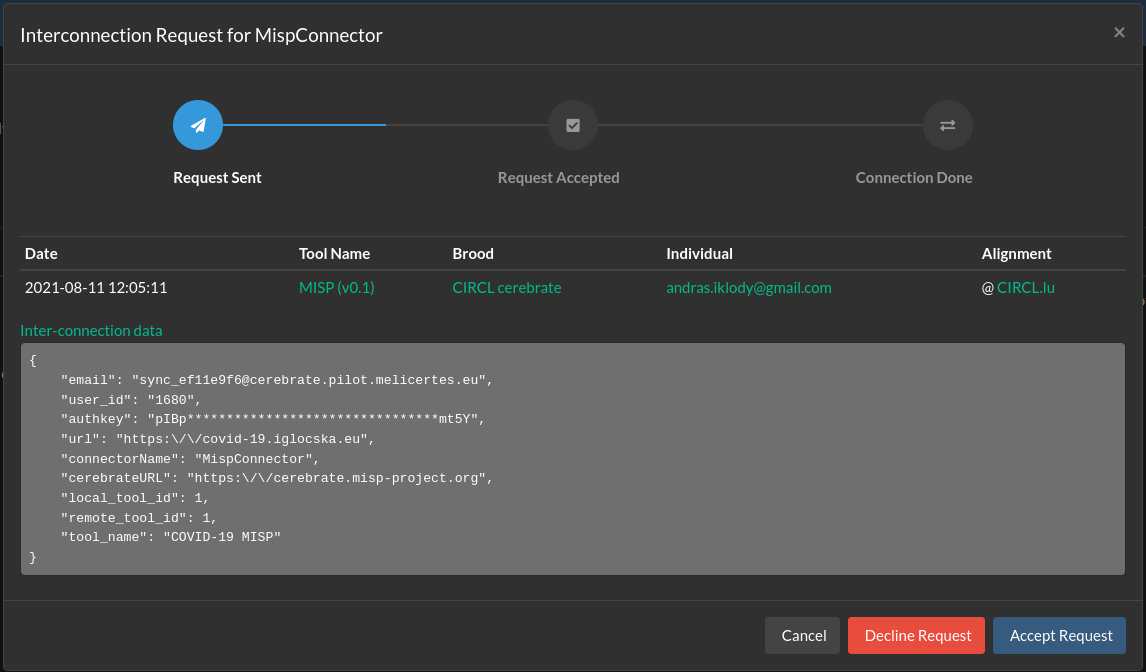
\includegraphics[width=0.98\linewidth]{pictures/connection_request.png}
    \end{center}
\end{frame}

\begin{frame}
\frametitle{What else does Cerebrate have?}
    \begin{itemize}
        \item Mailing list management
        \item ACL system
        \item Inbox system
        \begin{itemize}
            \item Inter-connection requests, enrolment requests
        \end{itemize}
        \item Tagging
        \item Update system
        \item Audit logs
        \item Open API
    \end{itemize}
\end{frame}

\begin{frame}
\frametitle{What else does Cerebrate have?}
    Cerebrate has \colorbox{black!90}{\color{white}\texttt{dark theme}} and \textbf{{\color{blue!70}m}{\color{red!70}o}{\color{purple!90}r}{\color{orange!70}e}}!
    \linebreak
    \begin{center}
        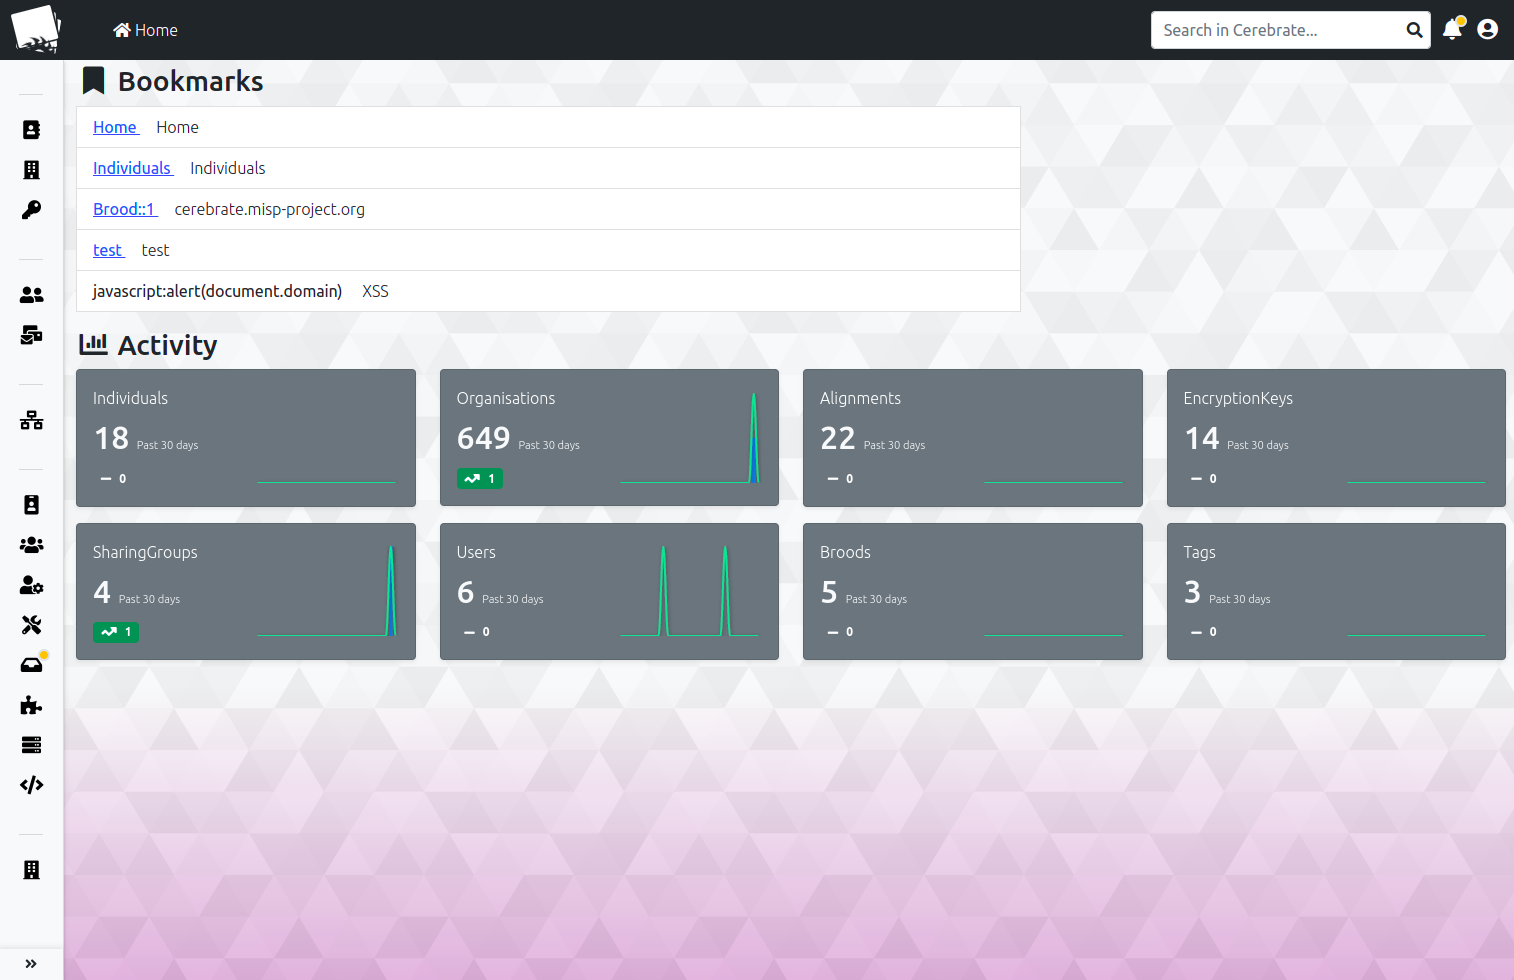
\includegraphics[width=0.42\linewidth]{pictures/theme-1.png}
        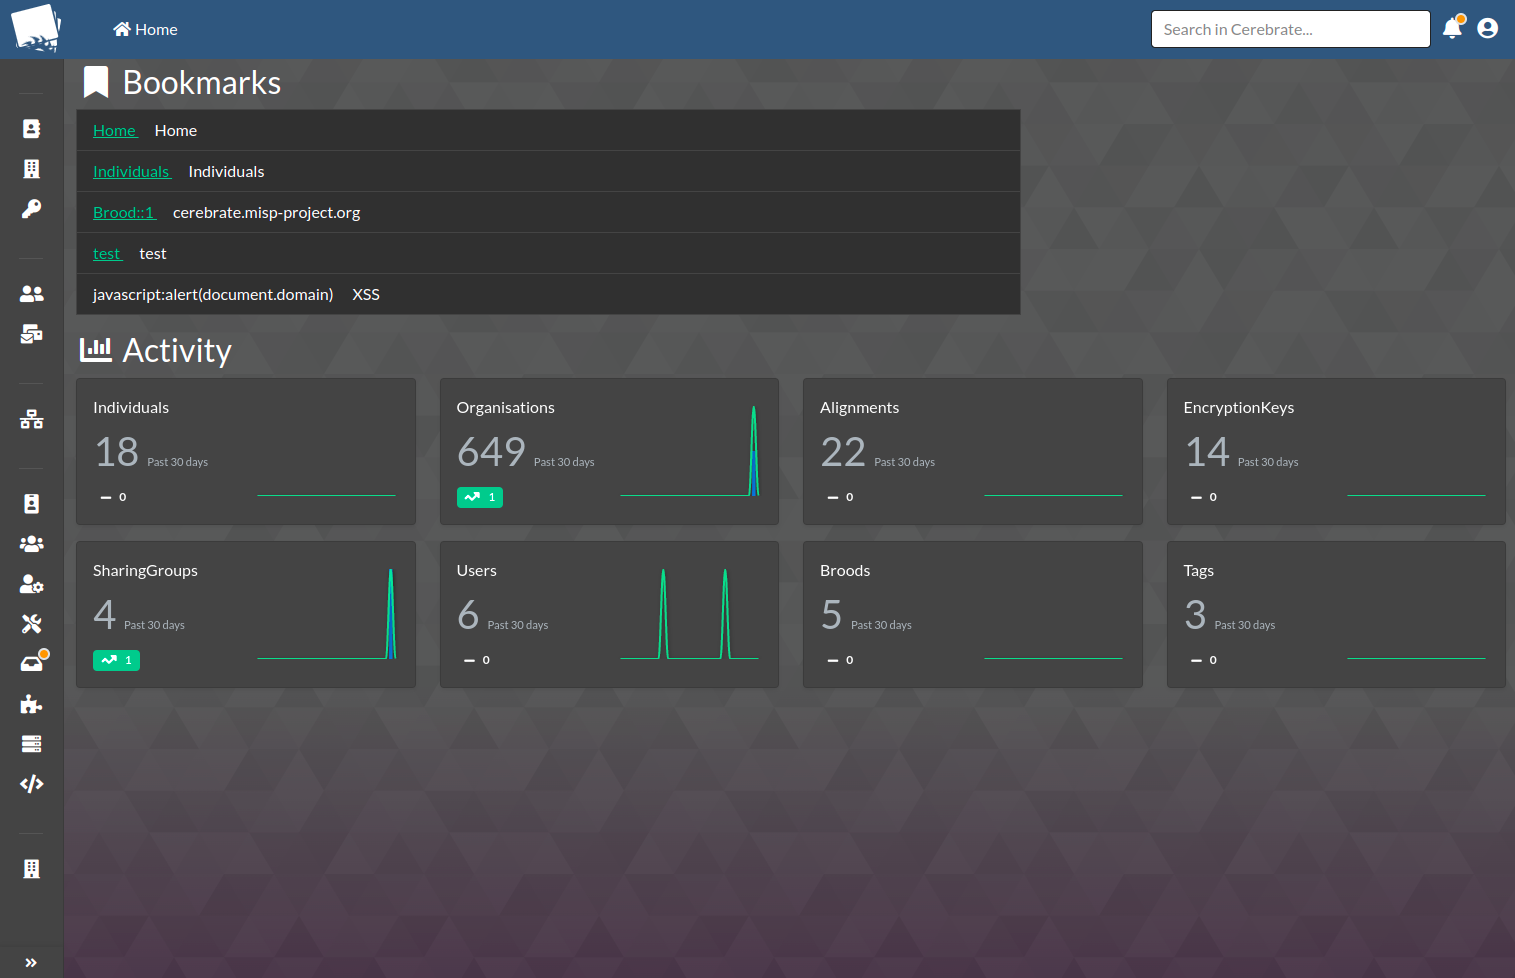
\includegraphics[width=0.42\linewidth]{pictures/theme-2.png}
    \end{center}
    \begin{center}
        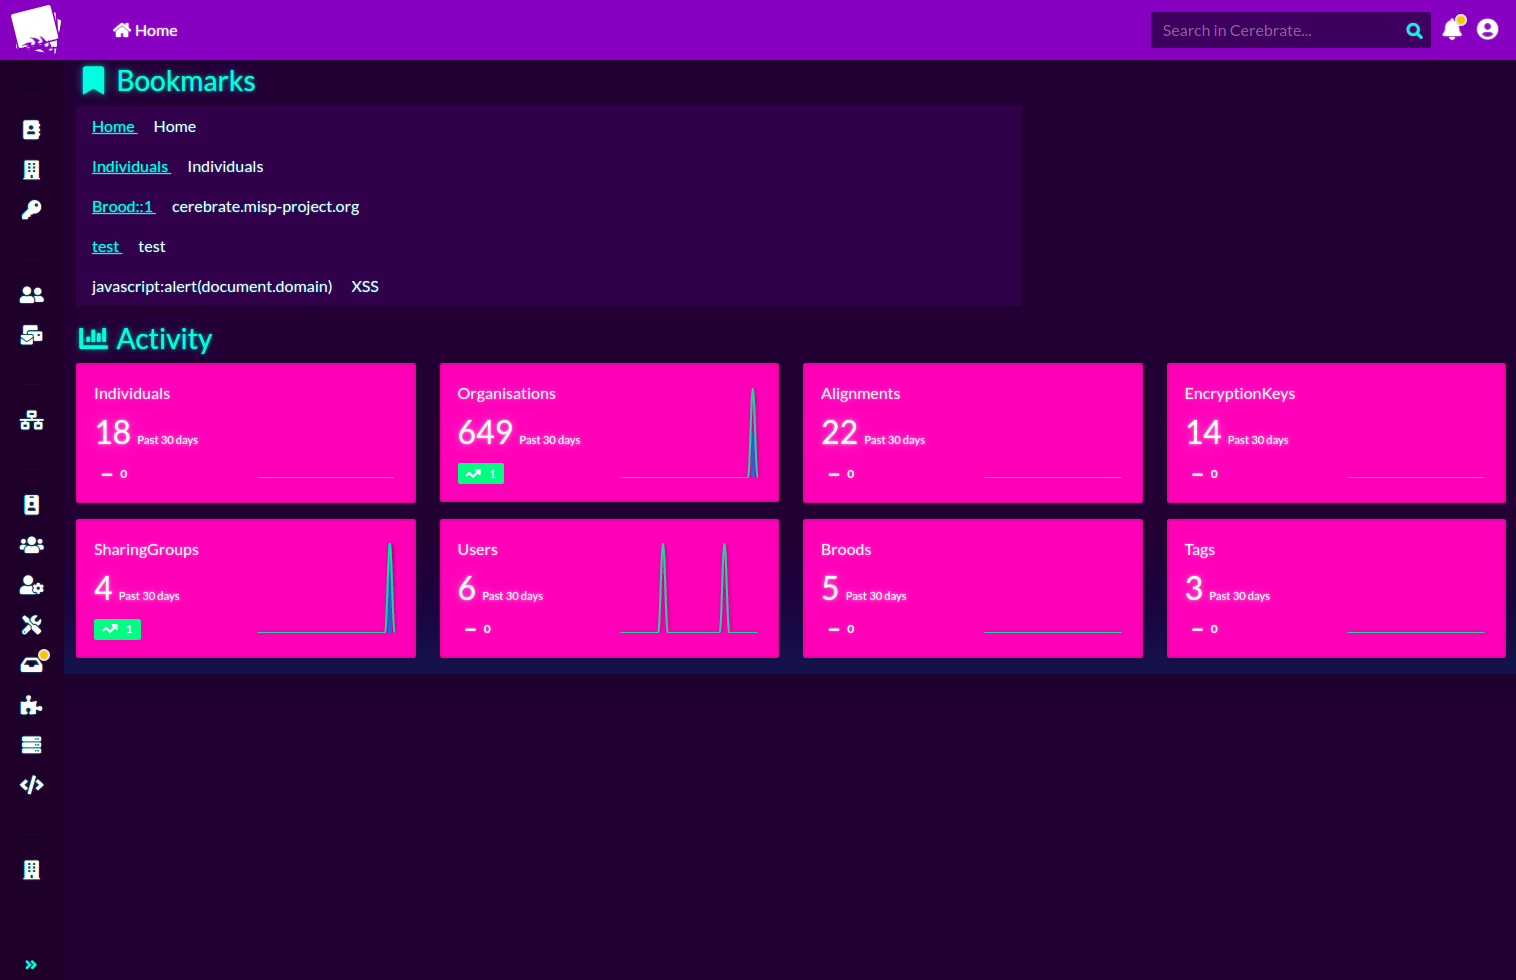
\includegraphics[width=0.42\linewidth]{pictures/theme-3.png}
    \end{center}
\end{frame}

\begin{frame}
\frametitle{Current roadmap}
    \begin{itemize}
        \item Data signing / validation
        \begin{itemize}
            \item Community centric PKI
            \item Enable data validation services for tools such as MISP
        \end{itemize}
        \item Integration with other tools
        \begin{itemize}
            \item Ticketing systems
            \item Tighter Mailing list integration (Mailman)
            \item Messaging App (Mattermost)
        \end{itemize}
    \end{itemize}
\end{frame}

\begin{frame}
\frametitle{Thanks!}
    \begin{itemize}
        \item Want to integrate your tool with Cerebrate?
        \begin{itemize}
            \item[ ] $\rightarrow$ Get in touch!
        \end{itemize}
        \item Want to have a live demo?
        \begin{itemize}
            \item[ ] $\rightarrow$ Get in touch!
        \end{itemize}
        \item Want to suggest features or integrations?
        \begin{itemize}
            \item[ ] That's right $\rightarrow$ Get in touch!
        \end{itemize}
    \end{itemize}
\end{frame}